In the following, data acquisition and database conversion are described. Content and related files, such as spreadsheets, scripts, and ontology files can be downloaded from the project website (http://www.cin.ufpe.br/\~{}integrativo).

\subsection{Sampling} 
Data related to 21 species\footnote{Giant panda, Bovine, white-tufted marmoset, dog, zebrafish, chicken, human, West Indian ocean coelacanth, African elephant, mouse, European domestic ferret, Nile tilapia, rabbit, chimpanzee, Sumatran orangutan, rat, Tasmanian devil, pig, Japanese pufferfish. Western clawed frog}, together with processes and by-products related to Hcy metabolism are retrieved from the UniProt and Ensembl websites\footnote{UniProt: Release 2015\_04, Ensembl Release 79, NCBI Taxonomy 2015AA.}. The ontologies GO, ChEBI and BTL2 are downloaded in OWL2 format\footnote{GO Revision 25527, ChEBI Release 127, BTL2 Release 8th march 2015, PR release 22nd may 2015, SNOMED CT July 31st 2014.}. 

For the creation of a subset from UniProt and Ensembl, UniProt data are filtered by the string ``homocysteine'', thus retrieving all Hcy-related data from UniProt/SwissProt+Trembl. From the obtained  212,156 records the ones with GO annotations, specified gene names and proteins as described by \cite{Selhub1999} are selected. From the resulting 1,716 records fragments, isoforms, or homologue entries are excluded. 
The resulting set includes the proteins Methionine synthase (MS), Methylenetetrahydrofolate reductase (MTHFR), Cystathionine beta-synthase (CBS), and Gamma-cystathionase (CSE). After removing records without Ensembl IDs, a final sample with 46 Hcy-related records is made available as a Microsoft Excel spreadsheet with the following tabular structure:
\begin{itemize}
	\item One Protein (e.g. \textit{CBS)};
	\item One Taxon (e.g. \textit{Rattus norvegicus}); 
	\item One to many GO biological processes (e.g., \textit{Blood vessel remodeling}) 
	\item One to many GO molecular functions (e.g., \textit{CBS activity}) 
	\item One to many GO cellular components (e.g., \textit{Cytoplasm}) 
	\item Zero to many phenotypes (e.g., \textit{Endocrine pancreas increased size}) 	
\end{itemize}

\subsection{Ontology mappings}
Root classes from GO, PR, ChEBI, NCBI Taxonomy, and SNOMED CT are included as subclasses of BTL2 nodes and tested for logical consistency (Fig. \ref{fig:HierarquiaURI}).
%In particular,  
%\begin{enumerate}
%	\item One or more references to GO classes in UniProt annotations for GO classes, such as 
%go:`\textit{Biological process}' go:\textit{Methylation} included as annotation for `\textit{Methionine 
%synthase}' in UniProt, as well as go:`\textit{Cellular component}' and go:`\textit{Molecular function}';
%	\item Reference to Proteins from PR directly as protein names in UniProt;
%	\item Database IDs from Ensembl in UniProt, and vice-versa;
%	\item Organism names as described in NCBI Taxonomy inside Ensembl and UniProt;
%	%	\item Gene products (mainly proteins) described in UniProt and Ensembl and available in PR.
%	\item Phenotypes according to Ensembl and included as a list of subclasses of btl2:\textit{Situation}, 
%alinged with \textit{Clinical finding} in SNOMED CT.
%\end{enumerate}
%\subsection{Technical aspects for ontology grounding} 
%The grounding process requires in-depth biology knowledge, insight into the way biological databases are populated, as well as ontology engineering skills, based on the understanding of upper level ontology principles and description logics.
%
%Aware that a straightforward, automatized “ontologization” of a database schema is not possible, the ontology engineer has to critically assess the pros and cons of competing modelling strategies. This must be perfor- med in a way that correctly accounts for the underlying biological reality on the one hand, and that provides enough expressiveness to address the use cases (formulated as competency questions), on the other hand.
%
%The following technical aspects were applied:   
%\begin{itemize}%
%
%\item Top-level classes and relations of the domain ontologies were aligned manually with the upper level ontology (cf. \ref{fig:HierarquiaURI}) with the Protégé v5 beta 17 ontology editor;
Mapping consistency is assured with the DL reasoner HermiT 1.3.8. For performance optimization, modules of external ontologies (GO, ChEBI, PR and SNOMED CT) are created, with the classes 
referred to in the selected database content as signature, using the Prot\'{e}g\'{e} plug-in Ontology Modularity \citep{Jiang2011}.  

All database objects are subjected to in-depth ontological analysis done by the authors. The content of a representative 
sample record is entirely modelled in Prot\'{e}g\'{e} as an OWL ontology, and tested for consistency and adequacy under BTL2. Once agreement is reached, this sample ontology is saved in OWL/XML format and manually dissected into code fragments, each of which is numbered and placed into a spreadsheet cell.  The code fragments are analysed to identify variable elements, i.e. class names specific to the underlying sample, encompassing protein, cellular component, biological function and other classes. All these names are then replaced by placeholders, thus yielding an ontology pattern specific to the data structure. 
The target ontology is then generated by iteratively filling the placeholders with the ontology class names from the database. This is done using a customized VBA script. This script has to account for the creation of named subclasses as well as for iterations over content of multi-valued fields.  
 
\begin{figure}[H]
	\centering
	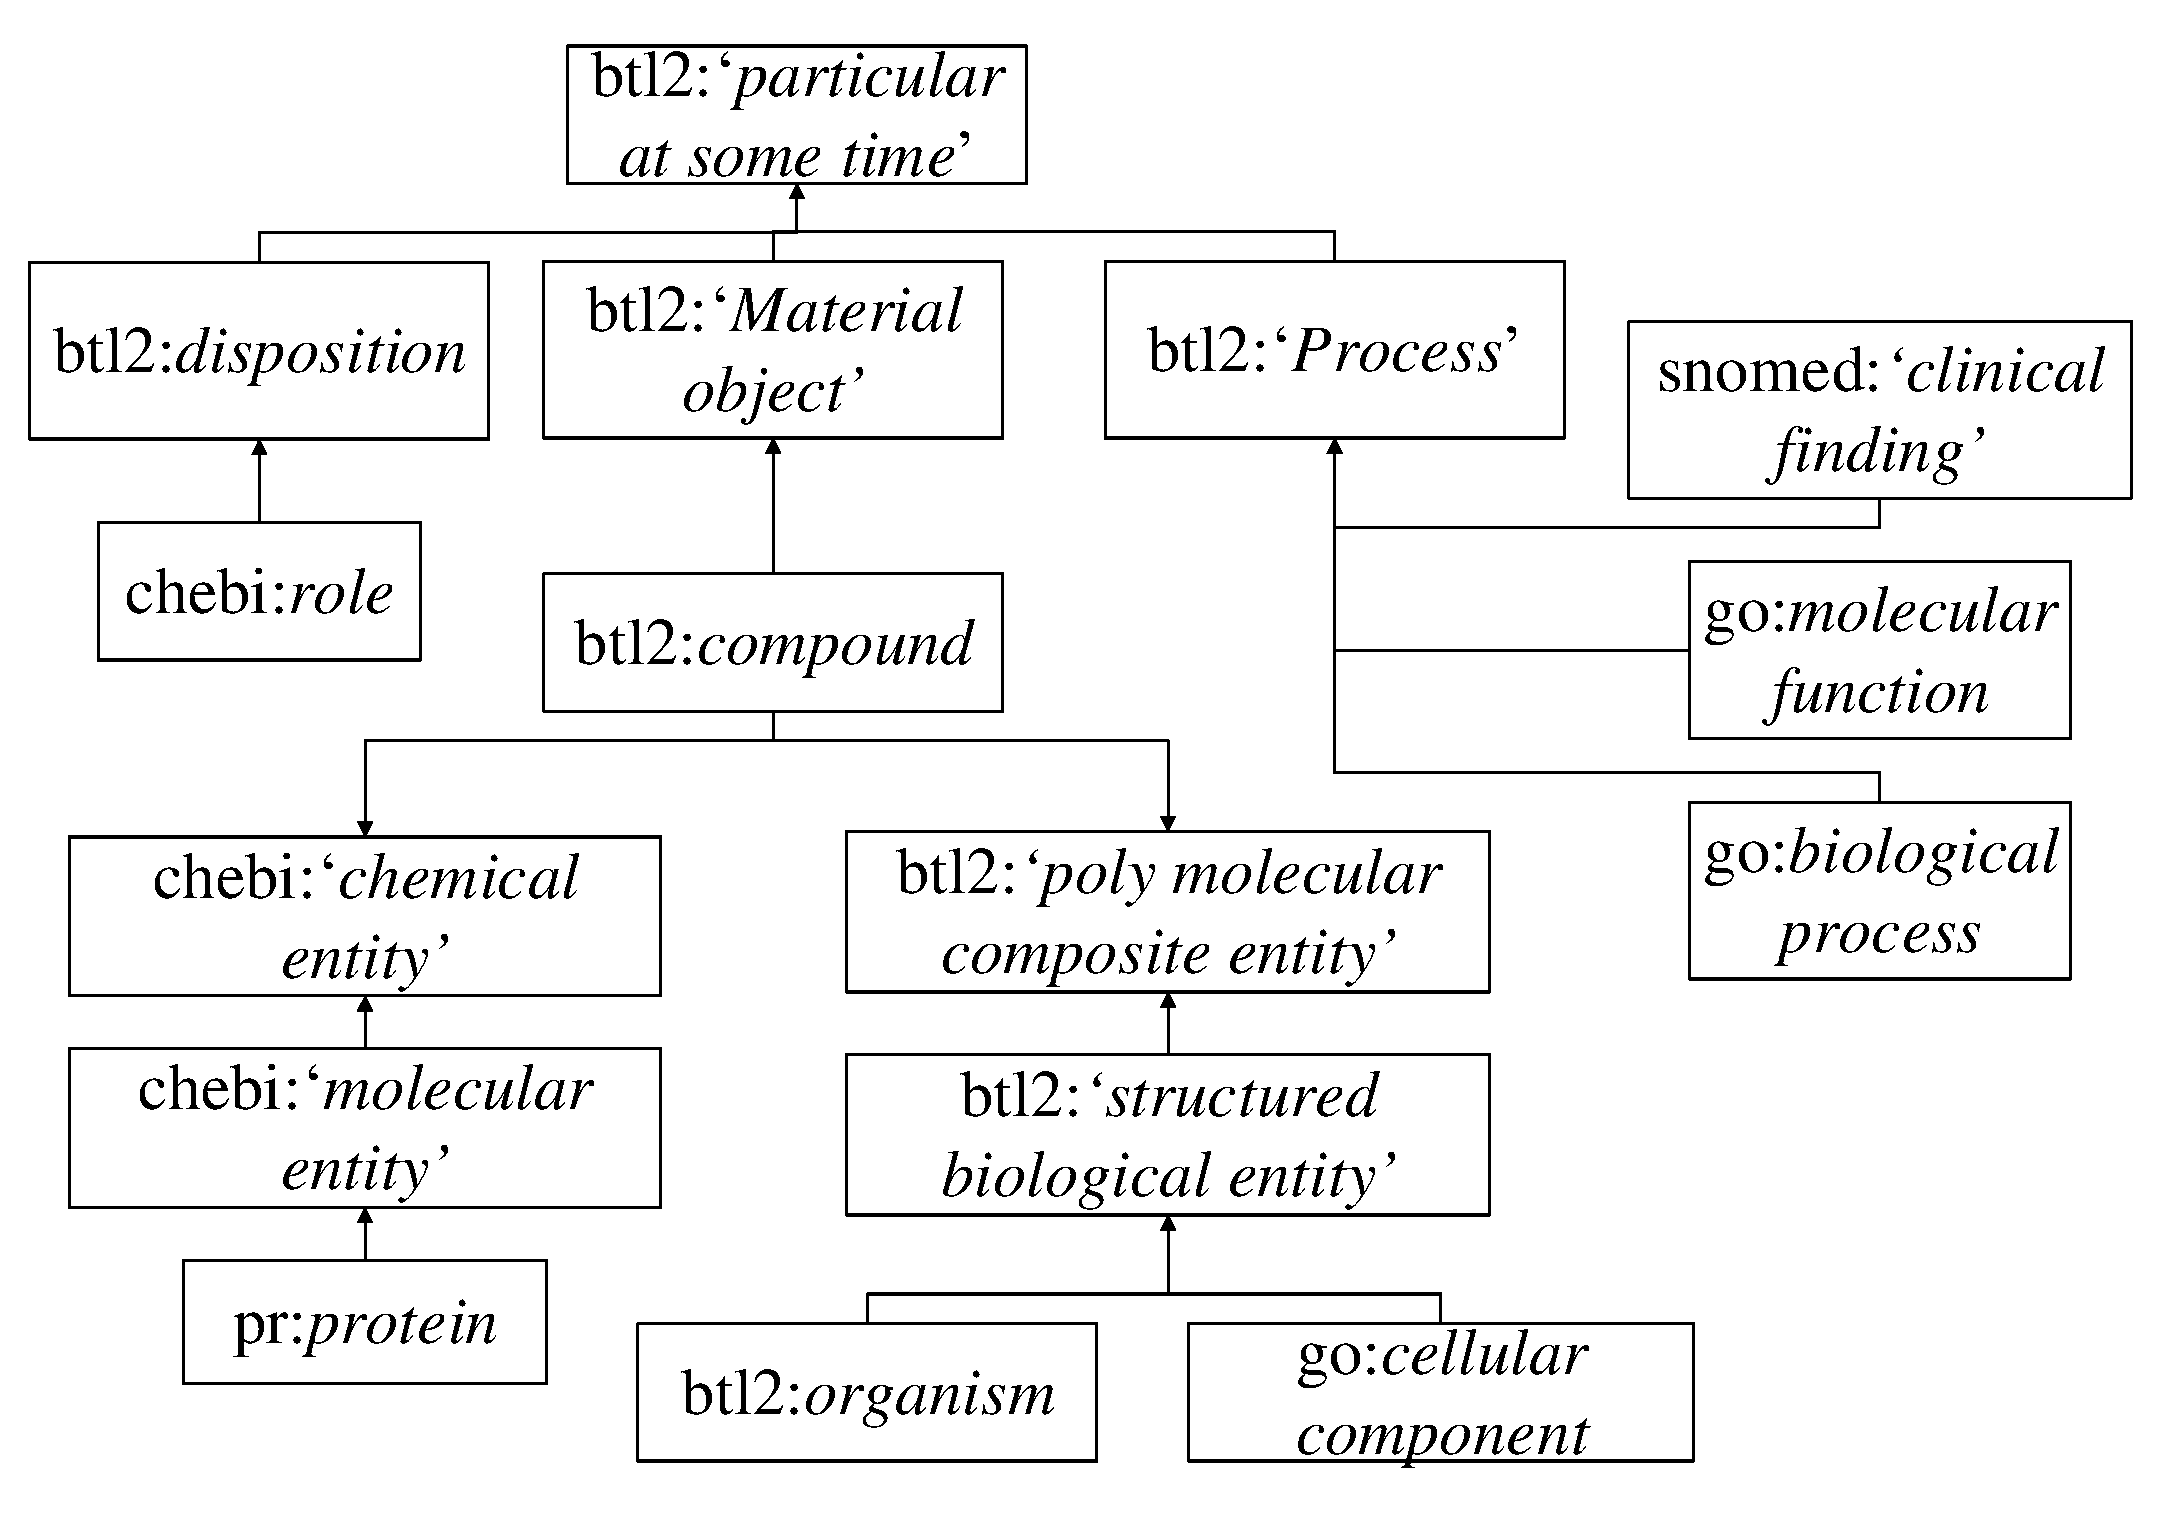
\includegraphics[width=0.9\linewidth]{./PIC/HierarquiaURI}
	\caption{Alignment of GO, ChEBI, SNOMED CT and PR under BTL2} 
	\label{fig:HierarquiaURI}
\end{figure}

%

\subsection{Evaluation methodology} \label{EvaluationMethodology}
The ontological content is evaluated by six competency questions (CQs),as introduced above. Formulated in English by the first author, a biologist, they are shaped according to how domain experts would query a biological database, and not how ontology engineers would interpret it, in order to be neutral regarding the internal structure of the ontology.
The translation of CQs into DL queries relies on the correct identification of query components that denote relations, referents, and the way how domain entities are related to one another (cf. section \ref{section:CQ}). To avoid biased judgements, this process is assessed by means of DL 
classification and retrieval of content from the axioms generated. %This is possible as CQs 
are rendered as DL queries and submitted to the final ontology.

 
Scalability is evaluated by artificially increasing the size of the ontology by a scaling factor $f$ $\in$ {1, 3, 10, and 30}. This is done programmatically, creating new classes suffixed by $i$ $\in$ {1, 2, \ldots, $f$}. Tangledness of these experimental ontologies is guaranteed by random assignment of \textit{i} in the axioms.  
The resulting ontologies are submitted to a DL reasoner to verify classification time. In addition, 
satisfiability time is measured, defined as the time it takes for validating a CQ 
against the derived model from the test ontology.
All tests are performed in Intel core i7-4510U laptop, with 8Gbytes of RAM, running Windows 10 (x64) and Java 8 (update 66, x64).
